\documentclass[border=4pt]{standalone}
\usepackage[T1]{fontenc}
\usepackage{amsmath}
\usepackage{mathpazo}
\usepackage{xcolor}
\usepackage{tikz}
\usetikzlibrary{positioning,arrows.meta}
\begin{document}
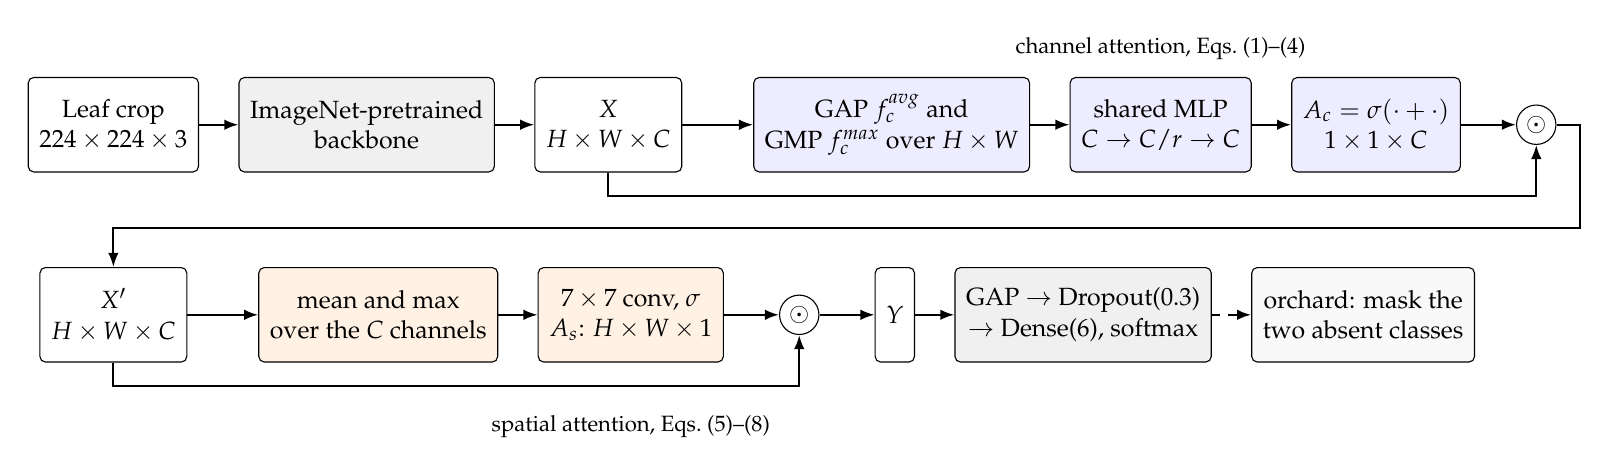
\begin{tikzpicture}[font=\small, node distance=5mm and 5mm,
  blk/.style={draw, rounded corners=2pt, align=center, minimum height=12mm, inner sep=4pt, fill=white},
  op/.style={draw, circle, inner sep=0.5pt, minimum size=5mm},
  arr/.style={-{Latex[length=1.8mm]}, thick}]
\node[blk] (in) {Leaf crop\\$224\times224\times3$};
\node[blk, right=of in, fill=gray!12] (bb) {ImageNet-pretrained\\backbone};
\node[blk, right=of bb] (X) {$X$\\$H\times W\times C$};
\node[blk, right=9mm of X, fill=blue!7] (cpool) {GAP $f^{avg}_c$ and\\GMP $f^{max}_c$ over $H\times W$};
\node[blk, right=of cpool, fill=blue!7] (mlp) {shared MLP\\$C \to C/r \to C$};
\node[blk, right=of mlp, fill=blue!7] (ac) {$A_c=\sigma(\cdot+\cdot)$\\$1\times1\times C$};
\node[op, right=7mm of ac] (m1) {$\odot$};
\node[blk, below=12mm of in] (Xp) {$X'$\\$H\times W\times C$};
\node[blk, right=9mm of Xp, fill=orange!10] (spool) {mean and max\\over the $C$ channels};
\node[blk, right=of spool, fill=orange!10] (conv) {$7\times7$ conv, $\sigma$\\$A_s$: $H\times W\times1$};
\node[op, right=7mm of conv] (m2) {$\odot$};
\node[blk, right=7mm of m2] (Y) {$Y$};
\node[blk, right=of Y, fill=gray!12] (head) {GAP $\to$ Dropout(0.3)\\$\to$ Dense(6), softmax};
\node[blk, right=of head, fill=gray!5] (mask) {orchard: mask the\\two absent classes};
\draw[arr] (in) -- (bb); \draw[arr] (bb) -- (X); \draw[arr] (X) -- (cpool);
\draw[arr] (cpool) -- (mlp); \draw[arr] (mlp) -- (ac); \draw[arr] (ac) -- (m1);
\draw[arr] (X.south) -- ++(0,-3mm) -| (m1.south);
\draw[arr] (m1.east) -- ++(3mm,0) |- ([yshift=5mm]Xp.north) -- (Xp.north);
\draw[arr] (Xp) -- (spool); \draw[arr] (spool) -- (conv); \draw[arr] (conv) -- (m2);
\draw[arr] (Xp.south) -- ++(0,-3mm) -| (m2.south);
\draw[arr] (m2) -- (Y); \draw[arr] (Y) -- (head); \draw[arr, dashed] (head) -- (mask);
\node[font=\footnotesize, above=1mm of mlp] {channel attention, Eqs.~(1)--(4)};
\node[font=\footnotesize, below=5.5mm of conv] {spatial attention, Eqs.~(5)--(8)};
\end{tikzpicture}
\end{document}
